\section{Implementation}
\label{sect:kegg_implementation}

The implementations for \mawapp and \keggapp similar in many ways, but they have
some important differences. Development on \keggapp was begun a year after
\mawapp and provided opportunities to improve on the interface, design, and
implementation of the pathway viewing app concept.

The improved design was made possible partially by new features introduced into
the iPad development environmeng in 2011 with the release of iOS 5. The most
important change was ``automatic reference counting,'' (ARC) which moves memory
management responsibility from the programmer to the compiler. (See section
\ref{sect:objc_memory} for more information on ARC).

\keggappp architecture consists of a few well-defined components. There are user
interface objects that present things like the master-detail interface, lists of
pathways, organism selection, etc. There are web service request classes that
make HTTP requests to the PathCase KEGG server, process the response, and notify
other objects of the results. There are graph rendering and interaction classes
similar to those found in \mawapp. Finally, there are encapsulated components
for specific functionality such as reading the ENZYME database and generating
dynamic layouts with Graphviz.

This section describes each of these components and how they differ from similar
components in \mawapp. Section \ref{sect:kegg_impl_ui} describes the user
interface for navigation the application. Section
\ref{sect:kegg_impl_web_services} describes how \keggapp interacts with the
\pathcasekegg web services. Section \ref{sect:kegg_impl_graph_view} covers the
pathway visualizer. Section \ref{sect:kegg_impl_enzyme} explains how the ENZYME
database \cite{enzyme-database} is used to look up and display extra information
about processes. Finally, Section \ref{sect:kegg_impl_graphviz} explains how the
Graphviz system \cite{graphviz} is used to generate dynamic layouts for graphs
that do not have curated frozen layouts.

\subsection{Navigation User Interface}
\label{sect:kegg_impl_ui}

Figure \ref{sect:kegg_impl_ui} shows a high-level representation of the user
interface components of \keggapp. Every class in the diagram except for the
\texttt{PCAppDelegate} application singletin is a view controller
(\ref{sect:cocoa_mvc}).

There are two kinds of edges in the diagram. \textbf{Present} edges are drawn
where one view controller causes another to be displayed in its content area.
For example, \texttt{UIViewController} shows the \texttt{PCMasterViewController}
in its sidebar area or popover (\ref{sect:ipad_container_views}), and the
\texttt{PCDetailViewController} in the rest of its content area. \textbf{Notify}
edges represent \emph{notifications} that are sent between objects.

A notification is an abstraction of message passing (\ref{sect:objc_objects}).
An object may \emph{register} for a notification of a certain name. When a
notification with that name is \emph{posted} by any object, the object that
registered for the notification is passed a message that was specified at
registration time. This message includes a \emph{notification object}, which may
contain additional data depending on the specific notification that was sent.
This system allows objects to send and receive events without storing
unnecessary references to other objects.

\begin{figure}[tbhp]
    \center{
        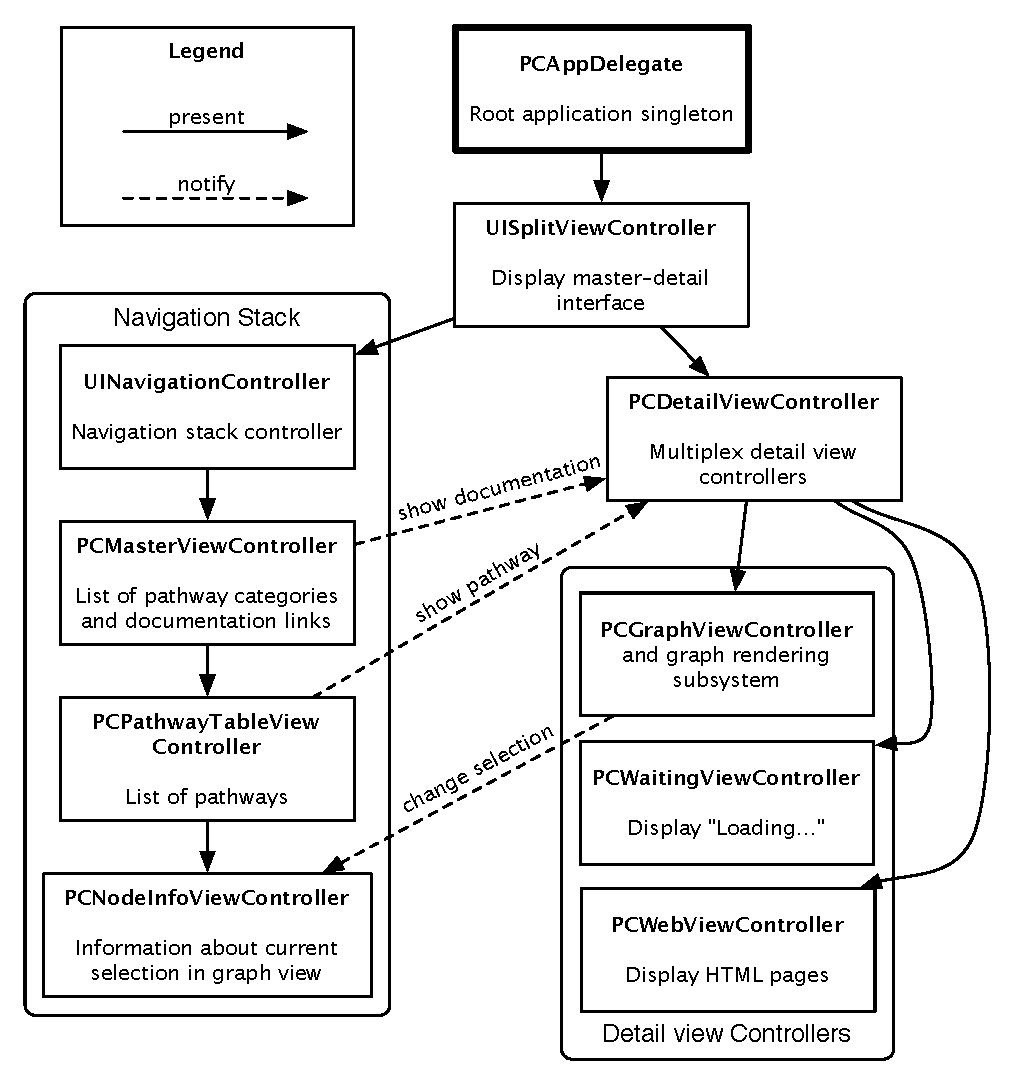
\includegraphics[width=\textwidth]{kegg/figures/architecture.pdf}}
    \caption{\label{fig:kegg_ui_arch} Components of the user interface. See
    \ref{sect:kegg_impl_ui} for more information about this diagram.}
\end{figure}

A good example of notifications can be found in \keggapp.
\texttt{PCMasterViewController}, a view controller included in in figure
\ref{fig:kegg_ui_arch}, shows a list of pathway categories and documentation
links (\ref{sect:kegg_interface}). Selecting a documentation link such as ``KEGG
Web Site'' posts a notification called \texttt{PCPageViewRequested} that
contains the URL of the corresponding web page, in this case
\href{http://www.kegg.com}{http:/\slash www.kegg.com\slash}.
\texttt{PCDetailViewController} has registered to receive this notification with
its method \texttt{pageViewRequested:}, which is implemented approximately like
this:

\begin{objc}
// Switch to a web view and show an HTML page in response
// to a notification
- (void)pageViewRequested:(NSNotification *)notification
{
    NSDictionary *info = [notification userInfo];
    [self.webViewController goToPage:[info objectForKey:@"url"]];
    [self switchToViewController:self.webViewController];
}
\end{objc}

This example is represented in figure \ref{fig:kegg_ui_arch} by the dashed arrow
``show documentation.''

\texttt{PCDetailViewController} responds to five different notifications, but
only two are shown in figure \ref{fig:kegg_ui_arch}. The rest have to do with
web services and pathway visualization interactions, which will be discussed
later in this section.

The remaining nodes in figure \ref{fig:kegg_ui_arch},
\texttt{PCPathwayTableViewController} and \texttt{PCNodeInfoViewController}, are
displayed in the master content area. The master view makes use of a
\emph{navigation stack} (see section \ref{sect:ipad_navigation}). The top item
on this stack is the \texttt{PCMasterViewController}, which pushes a
\texttt{PCPathwayTableController} onto the stack when a pathway category is
selected. When one of the pathways in that list is selected, a ``show pathway''
notification is posted, and a \texttt{PCNodeInfoViewController} is pushed onto
the stack. This is the view controller that displays information for the current
selection, so it responds to notifications sent by
\texttt{PCGraphViewController} about changes in the user's selection.

\subsection{Web Services}
\label{sect:kegg_impl_web_services}

\begin{figure}[hbt]
    \center{
        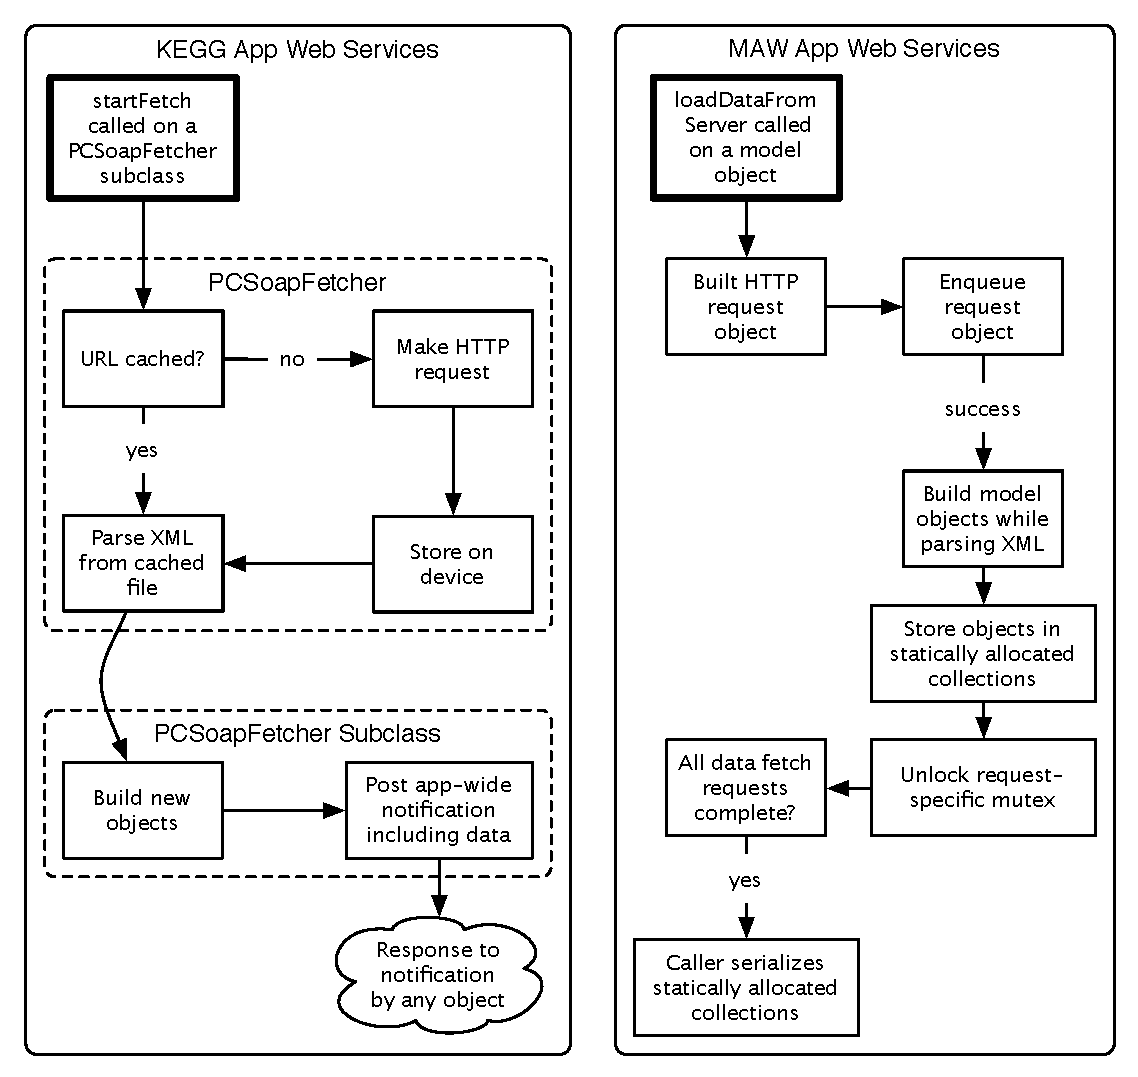
\includegraphics[width=\textwidth]{kegg/figures/web_services.pdf}}
    \caption{\label{fig:kegg_impl_web_service_differences} Side-by-side
    comparison of the typical life cycle of a \keggapp web service request and
    a \mawapp web service request.}
\end{figure}

There are four differences between the strategies of \mawapp and \keggapp
with respect to how web services are integrated into the application
architecture.

The first difference is that \keggapp does not download the entire PathCase
KEGG database at once. HTTP requests are made as new data is needed, and the
result is cached in the device's internal storage.

The second is in class hierarchy. \mawapp has methods in various data model
classes which are responsible for making an HTTP request and taking some action
based on its success or failure. \keggapp has a separate class for each web
service, named \texttt{PC<WebService>Fetcher}.

The third is how dependencies between requests are managed. \mawapp uses
mutexes to force the data update thread to wait before starting a request that
depends on a previous request. \keggappp web service classes fire events to
a central notification system when they have completed, and controller objects
check to see if any new web services should be invoked due to dependencies being
made available.

The fourth is in what sorts of transformations are done to the results of the
HTTP request. Unlike \mawapp, after the XML response has been parsed into
one or more KEGG internal objects, these objects are not serialized. In other
words, all objects generated by web services are built from the XML each time
they are needed. The XML response of the web service is the canonical
representation of the object.

These differences are summarized in figure
\ref{fig:kegg_impl_web_service_differences}.

This model of web services would not necessarily work better for \mawapp,
which needs quicker access to much more interdependent data. When the data model
is serialized, it is simple to load it and traverse complex relationships. The
data handled by \keggapp, on the other hand, is not very interdependent, so
it is simpler to make the web service requests on demand and turn the XML into
objects in memory on the fly.

\subsection{Pathway Visualizer}
\label{sect:kegg_impl_graph_view}

\subsubsection{Graph Renderer}

The \keggapp graph renderer is based on the \mawapp graph renderer, but the
\keggapp version is less dependent on the input data format and allows more
visual attributes to be changed after the graph is initially constructed.

Like \mawapp, the \keggapp graph representation has a \texttt{PCGraphNode} class
to represent a graphical node and a \texttt{PCGraphEdge} class to represent a
graphical edge. A \texttt{PCGraphModel} contains sets of these node and edge
objects to represent a single pathway visualization. The rendering method is
identical.

The main difference between the two visualization systems is in how the graphs
are constructed. In \mawapp, the node and edge objects have methods that set
graphical attributes such as shape, color, and label text based on a GML
expression (\ref{sect:smda_viz_data}). In that system, it is not possible to set
those attributes any other way. In \keggapp, the node and edge objects contain
no parsing code, but instead expose all graphical attributes as writeable
properties. The responsibility for parsing a graph definition and building a
graph model with the correct graphical attributes is moved to an external object
that is not part of the graph rendering system.

Node information that is relevant to the pathway visualization but is not
directly used for rendering has been moved to a \texttt{PCNodeInfo} class. Each
\texttt{PCGraphNode} instance references a \texttt{PCNodeInfo} instance which
contains the fields shown in table \ref{fig:kegg_node_info_fields}.

\begin{table}[htbp]
\centering
\begin{tabular}{ r | p{4in}}
    identifier  & Unique key to identify this node in the graph \\
    isProcess   & True if this node represents a process/reaction \\
    isMolecule  & True if this node represents a molecule \\
    reversible  & True if this node is a reaction and can be reversed \\
    label       & Text of this node's label \\
    ECNumbers   & All EC numbers associated with this node if it is a process
    \\
    moleculeRoles   & Dictionary mapping a process ID representing a
                        neighboring process node to this node's role in that
                        process (only used for molecules) \\
    processRoles    & Dictionary mapping a molecule ID representing a
                        neighboring molecule node to that node's role in this
                        process (only used for processes) \\
    neighborProcesses   & List of processes adjacent to this node if node is a
                            molecule \\
    neighboringProcessID    & Some molecules occur more than once in the same
                                visualization for cleaner layouts. This
                                identifier differentiates them. \\
    parentOrganisms & List of identifiers of organisms that contain this process
    \\
    allIdentifiers  & All identifiers associated with this node. Used as a
                        fallback if a node lookup fails. \\
\end{tabular}
    \caption{Fields of \texttt{PCNodeInfo}}
    \label{fig:kegg_node_info_fields}
\end{table}

\subsubsection{Organism Hierarchy}

The \keggapp pathway visualization includes the ability to select only a subset
of organisms to display information from. If reaction $R$ is present in
organisms $A$ and $B$ but not $C$, and organisms $A$ and $B$ are disabled, then
reaction $R$ will be dimmed in the visualization (\ref{sect:kegg_interface}).

\begin{figure}[hbtp]
    \center{
        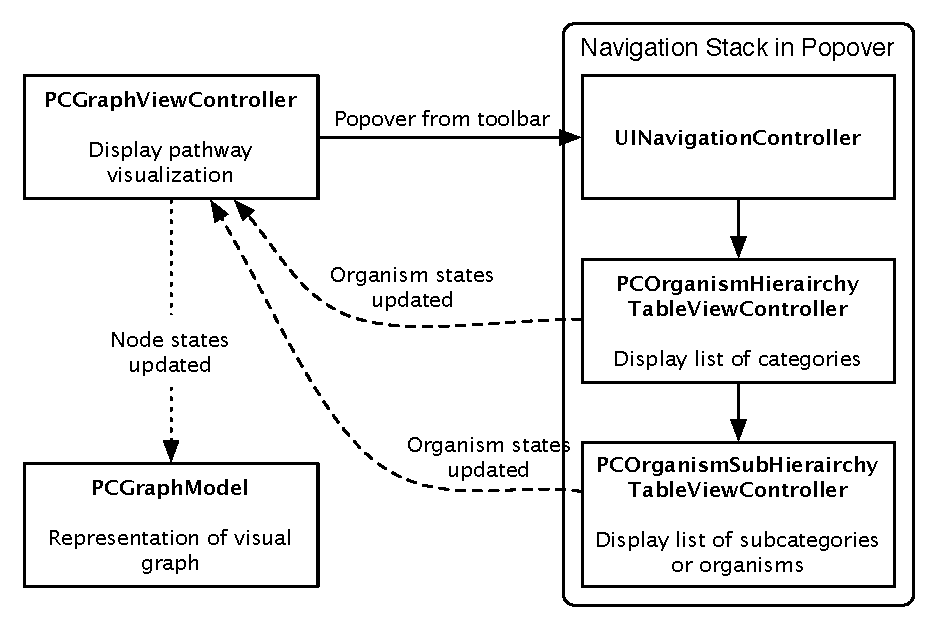
\includegraphics[width=5in]{kegg/figures/org_hierarchy_ui.pdf}}
    \caption{\label{fig:kegg_org_hierarchy_ui} Componentents of the organism
    hierarchy update process. See section \ref{sect:kegg_impl_graph_view} for
    more information.}
\end{figure}

The process of displaying the organism hierarchy is shown in figure
\ref{fig:kegg_org_hierarchy_ui} and described here. Selecting the toolbar
button in the upper right corner of the visualization view causes
\texttt{PCGraphViewController} to display a popover with a navigation stack. The
first item on this stack is a \texttt{PCOrganismHierarchyTableViewController},
which presents a table view containing hierarchical categories of organisms.
Tapping a row in the table view either pushes the subcategories of that category
onto the navigation stack if the row represents a subcategory, or it toggles the
enabled/disabled state of an organism if the row represents an organism. The set
of enabled organisms is then posted as a notification that is received by the
\texttt{PCGraphViewController}, which updates the \texttt{PCGraphModel} with the
enabled/disabled state of each individual node based on the enabled/disabled
state of the organisms.

The end result of this process is shown in figures
\ref{fig:kegg_screenshot_animals_only_list} and
\ref{fig:kegg_screenshot_animals_only_graph} in section
\ref{sect:kegg_interface}.

\subsubsection{Life Cycle of a Pathway Visualization}

\begin{figure}[htbp]
    \center{
        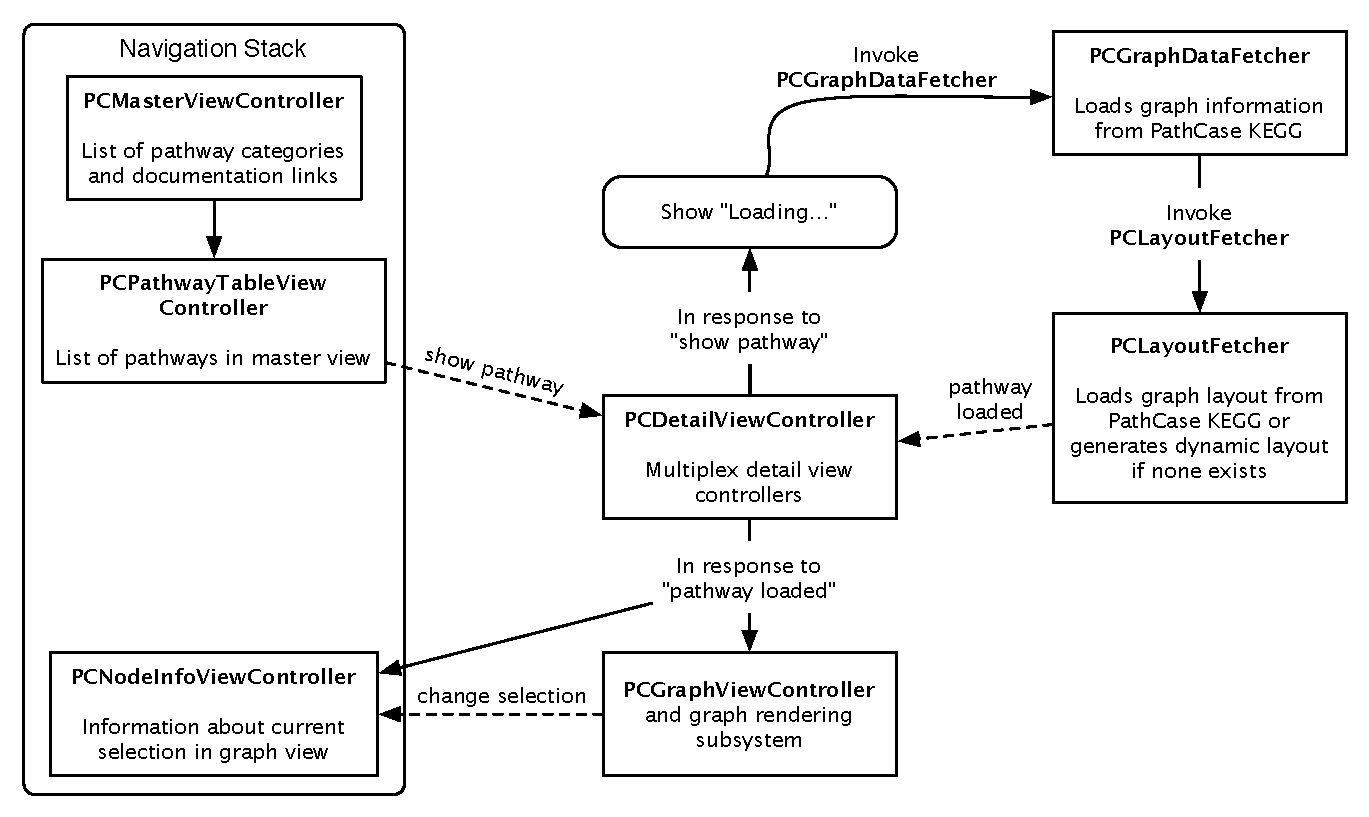
\includegraphics[width=\textwidth]{kegg/figures/viz_life_cycle.pdf}}
    \caption{\label{fig:kegg_viz_life_cycle} Life cycle of a pathway
    visualization. See section \ref{sect:kegg_impl_graph_view} for more
    information.}
\end{figure}

\subsection{Reading the ENZYME Database}
\label{sect:kegg_impl_enzyme}

The ENZYME database is provided in a flat text file format
\cite{enzyme:enzuser}. This format is not acceptable for random seeking
behavior, so it has been converted to a SQLite database \cite{sqlite:main} for
more efficient access. SQLite is a minimal implementation of SQL intended to be
used as a storage medium for single-instance applications \cite{sqlite:main}.

Each line in the ENZYME database begins with a two-letter code identifying the
type of data on the line \cite{enzyme:enzuser}. The rest of the line contains
the data. These are the different line codes according to the user manual:

\begin{objc}
ID  Identification                         (Begins each entry;
                                            1 per entry)
DE  Description (official name)            (>=1 per entry)
AN  Alternate name(s)                      (>=0 per entry)
CA  Catalytic activity                     (>=1 per entry)
CF  Cofactor(s)                            (>=0 per entry)
CC  Comments                               (>=0 per entry)
PR  Cross-references to PROSITE            (>=0 per entry)
DR  Cross-references to Swiss-Prot         (>=0 per entry)
//  Termination line                       (Ends each entry;
                                            1 per entry)
\end{objc}

\keggapp uses the description, alternate name, catalytic activity, cofactor, and
comments, ignoring the remaining fields.

The user manual uses this example to demonstrate the file format:

\begin{objc}
ID   1.14.17.3
DE   Peptidylglycine monooxygenase.
AN   PAM.
AN   Peptidyl alpha-amidating enzyme.
AN   Peptidylglycine 2-hydroxylase.
AN   Peptidylglycine alpha-amidating monooxygenase.
CA   Peptidylglycine + ascorbate + O(2) = peptidyl(2-hydroxyglycine) +
CA   dehydroascorbate + H(2)O.
CF   Copper.
CC   -!- Peptidylglycines with a neutral amino acid residue in the penultimate
CC       position are the best substrates for the enzyme.
CC   -!- The product is unstable and dismutates to glyoxylate and the
CC       corresponding desglycine peptide amide, a reaction catalyzed by
CC       EC 4.3.2.5.
CC   -!- Involved in the final step of biosynthesis of alpha-melanotropin and
CC       related biologically active peptides.
PR   PROSITE; PDOC00080;
DR   P08478, AMD1_XENLA ;  P12890, AMD2_XENLA ;  P83388, AMDL_CAEEL ;
DR   P10731, AMD_BOVIN  ;  P19021, AMD_HUMAN  ;  P97467, AMD_MOUSE  ;
DR   P14925, AMD_RAT    ;  Q95XM2, PHM_CAEEL  ;  O01404, PHM_DROME  ;
//
\end{objc}

A separate program was written to convert this file format into a SQLite
database. The program is called
\href{https://github.com/irskep/enzyme2sqlite}{enzyme2sqlite}
\footnote{\href{https://github.com/irskep/enzyme2sqlite}{https:/\slash
github.com\slash irskep\slash enzyme2sqlite}} and is implemented in the Python
3 programming language.

The program runs in two steps. The first step parses the text file format with a
simple state machine. The second step inserts the parsed data row by row
into a SQLite database. This database has fields that correspond directly to the
fields in the text file.

The program was invoked like this to generate the database used by \keggapp:

\begin{verbatim}
python3 enzyme2sqlite.py enzyme.dat -o enzyme.sqlite
\end{verbatim}

Access to the SQLite database in \keggapp is encapsulated in the
\texttt{EKEnzyme} class, which can open connections to the SQLite database and
query it for individual enzyme information. It can be used by calling
\texttt{[EKEnzyme enzymeForID:(NSString *)ECNumber]}, which returns an
\texttt{EKEnzyme} object with attributes for each field in its corresponding
ENZYME database entry. For example, to get the list of alternate names for
peptidylglycine monooxygenase, one would do this:

\begin{objc}
    // This class method will form the SQLite query
    // select * from enzymes where id = "1.14.17.3";
    EKEnzyme *myEnzyme = [EKEnzyme enzymeForID:@"1.14.17.3"];

    // The results have been read into myEnzyme
    NSLog(@"Alternate names: %@", [myEnzyme altNames]);
\end{objc}

\subsection{Dynamic Layouts with Graphviz}
\label{sect:kegg_impl_graphviz}

PathCase KEGG contains human-curated frozen layouts for some pathways, but not
all. In order to display the pathways without frozen layouts, \keggapp
uses the Graphviz library.

Graphviz is a system which, among other things, provides graph layout and
visualization functions \cite{graphviz}. It provides both command line and
programmatic interfaces for entering, laying out, and rendering graphs.

\keggapp encapsulates the layout functionality of the Graphviz library in a
class called \texttt{GVGraph}. An instance of this class represents a graph with
nodes, a label for each node, and one-directional edges that connect nodes.

To generate a layout, a \texttt{GVGraph} object must be created, and nodes and
edges must be added to it. This is accomplished by calling its methods
\texttt{addNodeWithID:label:} and \texttt{addEdgeWithHeadID:tailID:}. These
methods create internal \texttt{GVGraphNode} and \texttt{GVGraphEdge} objects
that represent the nodes and edges. These objects have no information about
color, shape, or other style attributes because those attributes are not
relevant to generating a layout.

Nodes and edges are added by calling methods on this class, which create
\texttt{GVGraphNode} and \texttt{GVGraphEdge} objects that contain only the
information that is important for generating a layout. They are completely
separate from the graph view node and edge objects that have additional
information about color and edge arrow shapes.

The dynamic layout is performed by calling the \texttt{computeLayoutWithEngine:}
method on the \texttt{GVGraph} instance. The argument to this function is a
constant representing either a spring-based or hierarchical layout engine. This
method converts the \texttt{GVGraphNode} and \texttt{GVGraphEdge} objects into
Graphviz's internal graph representation, asks Graphviz to generate a layout,
and reads the results back into the \texttt{GVGraphNode} and
\texttt{GVGraphEdge} objects. The caller may then read back the position data
from the \texttt{GVGraph} instance to use however it pleases.

To clarify these steps, here is the actual implementation of the dynamic layout
function in \keggapp, which applies a dynamic layout to the graph model
described in section \ref{sect:kegg_impl_graph_view}.

\begin{objc}
- (void)computeDynamicLayout
{
    GVGraph *g = [[GVGraph alloc] init];
    
    for (PCGraphNode *node in [self.nodes objectEnumerator]) {
        [g addNodeWithID:node.identifier label:node.label];
    }
    
    for (PCGraphEdge *edge in [self.edges objectEnumerator]) {
        [g addEdgeWithHeadID:edge.target.identifier tailID:edge.source.identifier];
    }
    
    [g computeLayoutWithEngine:GVLayoutEngineNeato];
    
    for (PCGraphNode *node in [self.nodes objectEnumerator]) {
        CGPoint position = [g positionForNodeID:node.identifier];
        node.position = position;
    }
}
\end{objc}
